\documentclass[11pt]{article}

%Sonderzeichen
\usepackage[T1]{fontenc}
\usepackage[utf8x]{inputenc} 

%Bilder
\usepackage{graphicx}
\usepackage{subfigure}
%Bild bennenen
\renewcommand{\figurename}{Bild}
%Nach Bild einrücken
\setlength{\parindent}{0pt}

%Stichwortverzeichnis
\usepackage{makeidx}
\makeindex

%Ränder
\usepackage{anysize}
\marginsize{2.4cm}{2.4cm}{2.2cm}{3cm}


%Sprache
\usepackage[german]{babel}
%\select@language{german}

%Numerierungstiefe
\setcounter {secnumdepth}{3}
\setcounter{tocdepth}{2}

%Verzeichnis verlinken
\usepackage{hyperref}

%Farben (Inhaltsverzeichnis)
\usepackage{color}
\definecolor{black}{rgb}{0,0,0}
\hypersetup{colorlinks, linkcolor=black}


%Kopf und Fusszeilen
\usepackage{fancyhdr}
\pagestyle{fancy} %vordefinierter Style
\fancyhf{}
%Kopfzeile
\fancyhead[L]{\nouppercase{\leftmark}}
\fancyhead[C]{TG 13/3 Projektdokumentation}
\fancyhead[R]{\today}
\renewcommand{\headrulewidth}{0.5pt}
\headheight 15pt
%Fusszeile
\fancyfoot[L]{Fabian Zeller }
\fancyfoot[C]{\thepage}
\fancyfoot[R]{Emanuel Hubenschmidt}
\renewcommand{\footrulewidth}{0.0pt}
\footskip 63pt

%Tabellen

\usepackage{tabularx}
\usepackage{float}
\floatplacement{figure}{H}

%Literaturverzeichnis
\usepackage{url}
\usepackage{cite}
\hypersetup{colorlinks, linkcolor=black}

%Mathematisch
\usepackage{amssymb}

%Code einbinden
\usepackage{listings} 
\usepackage{color}   
\usepackage[svgnames]{xcolor} 

\definecolor{mygreen}{rgb}{0,0.6,0}
\definecolor{mygray}{rgb}{0.5,0.5,0.5}
\definecolor{mymauve}{rgb}{0.58,0,0.82}

\lstset{language=Java}
\lstset{ %
  backgroundcolor=\color{white},   % choose the background color; you must add \usepackage{color} or \usepackage{xcolor}
  basicstyle=\footnotesize,        % the size of the fonts that are used for the code
  breakatwhitespace=false,         % sets if automatic breaks should only happen at whitespace
  breaklines=true,                 % sets automatic line breaking
  captionpos=b,                    % sets the caption-position to bottom
  commentstyle=\color{mygreen},    % comment style
  deletekeywords={...},            % if you want to delete keywords from the given language
  escapeinside={\%*}{*)},          % if you want to add LaTeX within your code
  extendedchars=true,              % lets you use non-ASCII characters; for 8-bits encodings only, does not work with UTF-8
  frame=single,	                   % adds a frame around the code
  keepspaces=true,                 % keeps spaces in text, useful for keeping indentation of code (possibly needs columns=flexible)
  keywordstyle=\color{blue},       % keyword style
  language=Java,                   % the language of the code
  otherkeywords={*,...},           % if you want to add more keywords to the set
  numbers=left,                    % where to put the line-numbers; possible values are (none, left, right)
  numbersep=5pt,                   % how far the line-numbers are from the code
  numberstyle=\tiny\color{mygray}, % the style that is used for the line-numbers
  rulecolor=\color{black},         % if not set, the frame-color may be changed on line-breaks within not-black text (e.g. comments (green here))
  showspaces=false,                % show spaces everywhere adding particular underscores; it overrides 'showstringspaces'
  showstringspaces=false,          % underline spaces within strings only
  showtabs=false,                  % show tabs within strings adding particular underscores
  stepnumber=2,                    % the step between two line-numbers. If it's 1, each line will be numbered
  stringstyle=\color{mymauve},     % string literal style
  tabsize=2,	                   % sets default tabsize to 2 spaces
  title=Codeausschnitt                 % show the filename of files included with \lstinputlisting; also try caption instead of title
}



\begin{document}

%Deckblatt

\title{Projektarbeit 2016\\TwitterStego-App}
\author{F.Zeller\\E.Hubenschmidt}
\maketitle
\newpage

%Inhaltsverzeichnis
\tableofcontents
\newpage

\section{Funktionsweise und Beschreibung}

\subsection{Beschreibung}
Die TwitterStego-App ist ein Programm für den PC welches Nachrichten in Bildern verstecken und wieder herausfiltern kann. Des weiteren kann man diese Bilder auf Twitter tweeten und auch nach Bildern auf Twitter suchen. Das Programm dient also zur verstecken Kommunikation über Twitter.

\subsection{Funktionsweise}

\begin{figure}[hbtp]
\centering
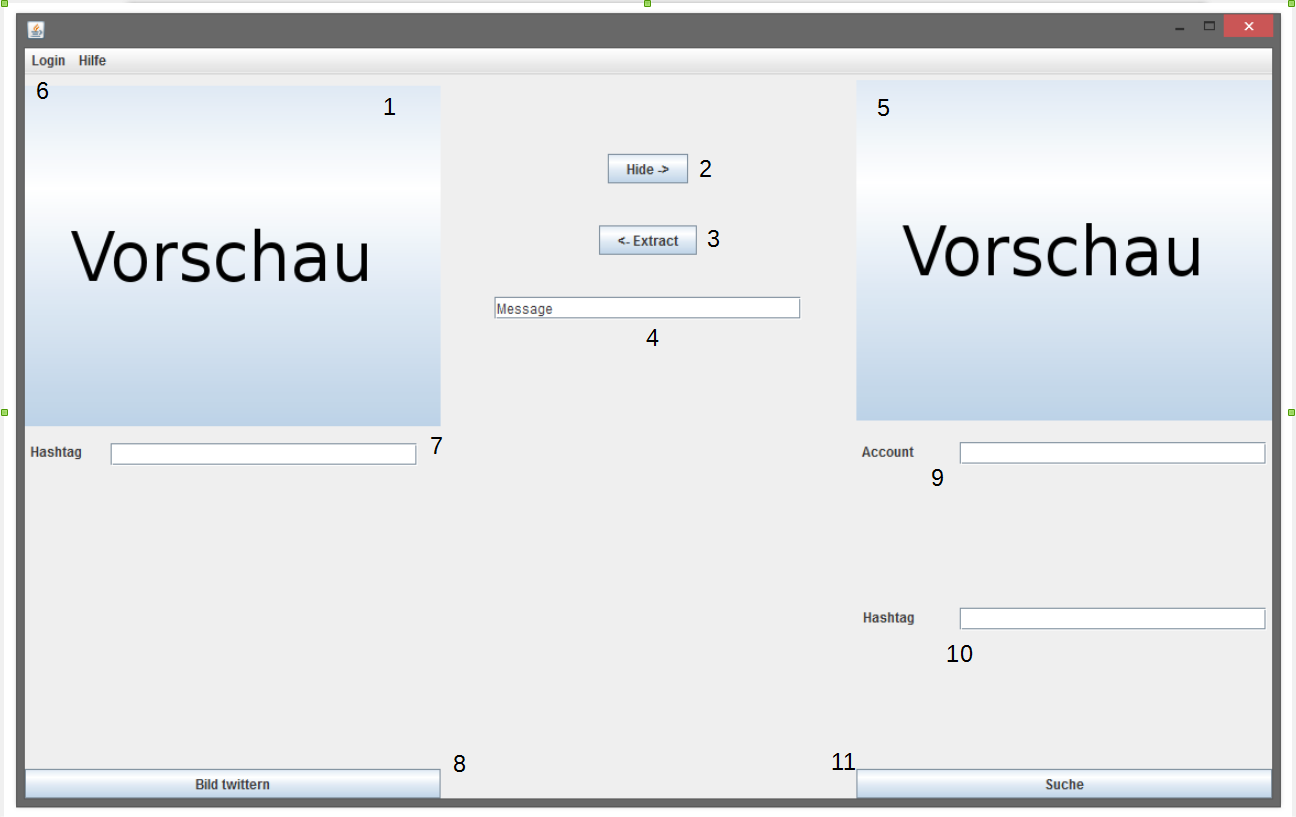
\includegraphics[scale=0.4]{GuiBeschriftet.PNG}
\caption{Die Oberfläche}
\end{figure}


\subsubsection{Nachrichten in Bildern verstecken}
Um eine Nachricht in einem Bild zu verstecken muss als erstes das Bild ausgewählt werden. Hierfür betätigt man die große Vorschau Fläche(1). Es öffnet sich ein Dateiexplorer und man kann ein Bild auswählen. Dieses Bild wird nun auf der Vorschaufläche angezeigt. 
\\
Als nächstes gibt man die zu versteckende Nachricht in das Message Feld(4) rechts neben der Vorschau ein. Um die Nachricht zu verstecken muss nur noch der Hide-Button(2) betätigt werden. Es öffnet sich wieder ein Dateiexplorer und man wählt den Speicherort für das Bild mit versteckter Nachricht aus.

\newpage

\subsubsection{Nachrichten aus Bildern filtern}
Um eine Nachricht aus einem Bild zu filtern muss das Bild ausgewählt werden. Hierfür betätigt man die rechte Vorschau Fläche(5). Mithilfe des Dateiexplorers wählt man das gewünschte Bild aus. Es erscheint nun in der rechten Vorschau. Sobald man den Extract-Button(3) betätigt wird die Nachricht im Message Feld(4) angezeigt. 

\subsubsection{Der Login}
Um auf Twitter zugreifen zu können muss man sich ersteinmal anmelden. Hierfür benötigt man den AccesToken, das AccesTokenSecret, den ConsumerKey sowie das ConsumerSecret. Diese vier Schlüsselbekommt man von Twitter. Man meldet sich hier: \url{https://apps.twitter.com/} mit seinem Twitter-Account an und folgt den Instruktionen. Sobald man seine Schlüssel hat wählt man in dem Menu Login(6) den Unterpunkt Neuer Login aus. Hier gibt man seine eben erworbenen Schlüssel sowie einen Speichername für diesen Login ein.
Ab sofort kann man auch die Twitterfunktionen der TwitterStego-App nutzen.

\subsubsection{Gespeicherte Logins}
Wenn man die vier Schlüssel eingibt muss man auch einen Namen eingeben. Mithilfe dieser Daten wird ein File erstellt welches nach schließen des Programms wieder aufgerufen werden kann. Dies wird mithilfe des Menüpunktes Login laden im Menü Login(6) bewerkstelligt. Somit muss man die Keys nicht wiederholt eingeben.


\subsubsection{Ein Bild Twittern}
Um ein Bild zu Twittern muss man nur einen beliebigen (optimal einen wenig oder nur eigen benutzten) Hashtag in das vorgesehene Feld(7) eintragen. Sobald der Button Bild-Twittern(8) betätigt wurde öffnet sich der Dateiexplorer und man kann das gewünschte Bild auswählen. 

\subsubsection{Ein Bild von Twitter suchen}
Um ein Bild von Twitter herunterzuladen muss man den Accountname des Publishers sowie den zum Bild zugehörigen Hashtag eingeben. Sobald man den Button Suche betätigt(11) öffnet sich der Dateiexplorer und man wählt den Speicherort aus. Das Bild wird gespeichert und automatisch in der rechten Vorschau(5) angezeigt. 



\newpage
\section{Steganographie}
Die Steganographie ist ein Unterkapitel der Kryptographie. Ihr Ziel ist es Nachrichten in einem andern Medium zu speichern. Der begriff leitet sich aus dem griechischen ab und bedeutet ''bedeckt schreiben´´. Erstmals wurde diese verfahren um 400 v.Chr. verwendet, indem man z.B. Nachrichten auf die Innenseite von Wachstafeln ritzte und dort drüber dann Wachs goss.\\
Heutzutage wird die Steganographie hauptsächlich in digitalen Median verwendet. Hierzu bieten sich besonders Bilder oder Audiodateien an. Ein digitales Bild, z.B. eine png-Datei, besteht aus einer Matrix von Werten. Jeder Wert stellt einen Pixel da, welcher sich wiederum aus 4 Werten zusammensetzt, nämlich dem rot, grün, blau und Alpha Wert. Diese sind jeweils 8 Bit lang, somit ergibt sich eine 32-Bit lange Zahl. Um nun eine Nachricht darin verstecken zu können, muss man diese Werte so manipulieren, dass ohne das Original, die Manipulation nicht auffällt. Dazu wird die Nachricht zuerst in eine binäre Darstellungsform (z.B. binärer ASCII-Code) gebracht. Anschließend werden die Last Significant Bit einer Farbe durch die Bits der Nachricht ersetzt. Der Alpha-Wert ist hierfür nicht geeignet, denn er gibt die Transparenz eines Pixels an. Mit dem bloßen Auge wäre zwar trotzdem kein Unterschied zu erkennen, allerdings ist der Alpha Wert normalerweise für jeden Pixel auf 255 (nicht Transparent), wodurch eine Manipulation auffallen würde.\\
In unserm Programm gibt eine Bitfolge von 8 Einsern in den ersten 8 Pixeln eines Bildes an, das sich in dem Bild eine Nachricht versteckt. Das Programm liest dann solange alle LSBs der Pixel, bis es auf zuerst 8 Nullen und dann auf 16 Einsen trifft. Dies bedeutet, dass die Nachricht zu ende ist. Die 8 Nullen sind dazu da, damit nicht die Einser, die zu einer Nachricht gehören als Einser dieser Schluss Bitfolge gezählt werden. Zum Beispiel ist ein Fragezeichen in binären ASCII Code eine 0011 1111. Wenn direkt darauf die 16 Einser folgen würden nur die zwei Nullen zur Nachricht zählen und den Rest als Schluss Signal.


\newpage
\section{Entwicklungshergang}

\subsection{Zeitliches Limit}

Da das Schulprojekt auf nur 3 Wochen begrenzt war mussten wir uns bei der Gestaltung der TwitterStego-App beschränken. Bei der Steganographie wird eine Nachricht versteckt aber mithilfe der Kryptographie eigentlich noch zusätzlich verschlüsselt. Aufgrund der kurzen Zeitspanne haben wir beschlossen diese Funktion auszulassen. Auch wollten wir zu Anfang weitere Twitter-Funktionen einfügen wie mehrere Bilder auf einmal zu suchen und diese in einer Datenbank zu speichern. Darin hätte man Teilnachrichten verstecken und diese dann mithilfe der TwitterSego-App zusammenfügen können. Trotzdem sind wir mit dem Ergebnis zufrieden da die Grundfunktionen gewährleistet sind.

\subsection{Aufteilung der Aufgaben}

Da wir zu zweit mithilfe von GitHub an dem gleichen Projekt arbeiten konnten war die Teilung der Aufgaben sehr einfach. Anfangs beschäftigte sich Herr Hubenschmidt mit dem Verstecken von Nachrichten in Bildern und Herr Zeller mit der Verbindung zu Twitter. Als diese großen Teilpunkte erfüllt waren verband Herr Hubenschmidt diese und Herr Zeller gestaltete die Grafische Oberfläche.

\newpage
\subsection{Codeausschnitte}

\subsubsection{Steganographie Code}
\begin{lstlisting}[frame=single]  % Start your code-block

public BufferedImage hideText(String text, File img) throws IOException {

		BufferedImage bufferedImage = ImageIO.read(img);
		int w = bufferedImage.getWidth();
		int h = bufferedImage.getHeight();


		if (w*h -16 <= text.length() * 8) {
			gui.error("Text ist zu lang");
			return null;
		}
		
		int stelle = 0;

		int[] textBits = new int[text.length() + 8];
		textBits = bitsInText(text);

		for (int i = 0; i < h; i++) {
			for (int j = 0; j < w; j++) {
				if (textBits.length <= stelle) {
					break;
				}

				bufferedImage.setRGB(j, i, setLastBit(bufferedImage.getRGB(j, i), textBits[stelle]));
				stelle++;

			}
		}

		return bufferedImage;

	}


\end{lstlisting}

\underline{\textbf{Beschreibung:}}\\
Diese Methode versteckt eine Nachricht in einem Bild.\\

\newpage
\subsubsection{Twitter Code}
\begin{lstlisting}[frame=single]  % Start your code-block

public String getTweetandMediafromHash(String hash, String user) {

		String returnvalue = null;

		try {
			ResponseList<Status> timeline = twitter.getUserTimeline(twitter.showUser(user).getId());

			for (Status status : timeline) {
				for (HashtagEntity hashtags : status.getHashtagEntities()) {
					if (hashtags.getText().equals(hash)) {
						for (MediaEntity mediaEntity : status.getMediaEntities()) {
							returnvalue = mediaEntity.getMediaURL();
						}
					}
				}
			}
		} catch (IllegalStateException e) {

			e.printStackTrace();
		} catch (TwitterException e) {

			e.printStackTrace();
		}

		return returnvalue;

	}
\end{lstlisting}

\underline{\textbf{Beschreibung:}}\\
Diese Methode sucht auf Twitter nach einem Bild.\\

\newpage
\subsubsection{Gui Code}

\begin{lstlisting}[frame=single]  % Start your code-block

protected void btLoadLoginClicked() {
			
			String url = LoginData.class.getResource("").toString();
			url = url.substring(5, url.length());
			url = url.replace("Twitter/", "") + "LoginData/";
			File folder = new File(url);
			File[] listOfFiles = folder.listFiles();
			Vector<String> fileNames = new Vector<String>();
			for (int i = 0; i < listOfFiles.length; i++) {
				if (listOfFiles[i].isFile() && listOfFiles[i].getName().contains(".bin")) {
					fileNames.add(listOfFiles[i].getName().replace(".bin", ""));
				}
			}
			String[] fileNamesArray = fileNames.toArray(new String[0]);
			String fileName = (String) JOptionPane.showInputDialog(null, "Auswahl", "Auswahl",
					JOptionPane.QUESTION_MESSAGE, null, fileNamesArray, fileNamesArray[0]);
			url = url + fileName + ".bin";
			try {
				loginData = loginData.loadLoginData(url);
			} catch (FileNotFoundException e) {
				e.printStackTrace();

			} catch (ClassNotFoundException e) {
				e.printStackTrace();

			} catch (IOException e) {
				e.printStackTrace();

			}
			twitterLogin.setLoginData(loginData);
			twitterLogin.reConfiguration();
			loginDatenGesetzt = twitterLogin.checkLogin();
	
	}

\end{lstlisting}

\underline{\textbf{Beschreibung:}}\\
Diese Methode wird aufgerufen wenn ein bestimmter Button betätigt ist.\\


\newpage
\section{Reflexion}

Durch schon vorherige zusammenarbeitet fiel uns diese Projekt nicht allzu schwer. Es war etwas Einarbeitungszeit in bestimmte Themen wie die Twitter4J Bibliothek oder die Steganographie nötig, diese stellte aber keine allzu großen Hürden dar. Mit dem Resultat sind wir beide zufrieden. Es gab nie oder keine Unstimmigkeiten und Probleme wurden schnell diskutiert und behoben. Alles in allem ein gelungenes 3 Wochen Projekt an dem wir viel Spaß hatten.





\end{document}